\chapter{Traceable Physics Models}
\label{chap:physics}

This thesis also contributes computational implementations of several key physics models for aircraft design that are traceable within the example code transformations framework introduced in Section \ref{sec:aerosandbox}, AeroSandbox. The broad motivation for this contribution stems from the observation that ``ease-of-model-implementation'' has historically proven to be one of the most important factors for determining whether an MDO paradigm can achieve use in industry. More specifically, the goals of this contribution are to:

\begin{enumerate}
    \item Stress-test the feasibility of code transformations in practice—how much added user effort and expertise is required to bring typical engineering analyses into a code-transformations-based MDO tool? To what extent can existing code be used as-is? Finally, the thesis aims to identify any specific computational elements that cause ``pain points'' when attempting to make an analysis traceable.
    \item Jump-start future applied research by providing a set of modular, plug-and-play analyses that can be used to quickly build a variety of aircraft design optimization problems. Since the long-term goal of this research direction is to establish whether the proposed MDO paradigm improves practicality, many practical aircraft design problems must be posed. Creating a set of modular general-purpose building blocks reduces the need to write similar analysis code repeatedly, saving time for designers.
\end{enumerate}

To achieve these goals, this thesis contributes the traceable implementations of the analyses given in Table \ref{tab:models_to_contribute}. This set of analyses was deliberately chosen to be mathematically diverse, spanning a wide range of common code patterns in scientific computing. The types of attributes that each analysis is intended to stress-test are given in the right-most column of Table \ref{tab:models_to_contribute}.

\begin{table}[H]

    \centering
    \caption{A list of aircraft design analyses that the thesis implements within a code transformations framework. The middle column lists the non-traceable tools for each analysis that are commonly used in industry today. The right-most column lists the computational attributes that each analysis is intended to stress-test.}
    \label{tab:models_to_contribute}
    \setstretch{1.25}
    \begin{tblr}{
        colspec={@{} X X X @{}},
        row{1}={font=\bfseries},
        hline{3-6}
    }
        \toprule
        Analysis To Contribute                            & Non-Traceable Analogue                                                        & Tests tracing through\ldots                                                                                                 \\ \midrule
        Vortex-Lattice Method Aerodynamics Analysis       & AVL \cite{avl}                                                                & An aerospace geometry engine and discretization; large, vectorized matrix methods, like linear solves                       \\
        Nonlinear Lifting Line Aerodynamics Analysis      & Phillips \& Snyder \cite{phillips_modern_2000}, Reid \cite{reid_general_2020} & Nonlinear systems of equations (i.e., implicit), which often lead to value-dependent code execution (via convergence loops) \\
        Workbook-style Aerodynamics Buildup               & USAF Digital DATCOM \cite{datcom}                                             & Table lookups, large amounts of conditional logic (yielding a wide, branching graph), and scalar-heavy math                 \\
        Rigid-Body Equations of Motion                    & ASWING (dynamics) \cite{aswing}                                               & Ordinary differential equations, which are often implemented in a loop-heavy way (yielding a deep graph)                    \\
        Linearized Aircraft Stability Modal Decomposition & AVL \cite{avl}                                                                & More advanced matrix methods, such as an eigenvalue decomposition                                                           \\
        \bottomrule
    \end{tblr}

\end{table}

These traceable implementations offer value within the context of the thesis itself (in stress-testing the practicality of code transformations), but they also have value as a standalone contribution to the aircraft design community—even outside of design optimization. Because of the mixed-backend numerics library described in Section \ref{sec:code_syntax}, these analyses can be used independently from the design optimization context of AeroSandbox if desired. In such cases, however, they still can retain certain runtime benefits from the code transformations framework, if desired by the user. For example, a traceable workbook-style aerodynamics buildup would seamlessly enable GPU-accelerated evaluations and automatic vectorization, offering significant speedups; an example application might be real-time performance estimation for model predictive controllers or flight simulation.


\section{Vortex-Lattice Method Aerodynamics Analysis}

\subsection{Method Overview}
\label{sec:vlm_theory}

The vortex-lattice method (VLM) is a low-fidelity aerodynamics analysis used to model the inviscid 3D flow field around a system of lifting surfaces (e.g., wings). It is one of the most common conceptual-level aerodynamics analyses used in aircraft design, as it is computationally inexpensive and interpretable. Common tools that implement the VLM include AVL \cite{avl} and XFLR5 \cite{xflr5}.

A VLM analysis is based on classical potential-flow theory. Because this flow field model is a linear partial differential equation, it can be quickly solved using a boundary-element method representation by superimposing Green's-function kernels. These kernels model disturbances in the flow field that are induced by the lifting surfaces. In a VLM analysis, these kernels are modeled as a collection of \emph{horseshoe vortices} that are distributed along the wing in a regular lattice pattern. Each horseshoe vortex is a connected polyline of uniform-strength vortex filaments, with three segments: a bound vortex on the wing, and two trailing legs extending downstream to infinity\footnote{These trailing legs extend to the far-field Trefftz plane. In theory, these trailing legs should follow the local flow direction (and hence be ``force-free'' by the Kutta-Joukowski theorem), but often they are simply extended directly backwards which simplifies induced velocity computation and removes the need for an iterative wake relaxation.}. (In practice, a fourth leg consisting of a far-downstream ``starting vortex'' can be imagined to close the horseshoe vortex, which forms a ring vortex and thus satisfies the Helmholtz vortex theorems.) The Kutta condition is naturally satisfied, as the only place where the wing can shed vorticity is at the trailing edge (due to placement of the trailing legs).

Each horseshoe vortex has an initially-unknown strength, and the vorticity associated with each vortex creates an induced velocity that affects the global flowfield. To solve for these $N$ unknown vortex strengths, $N$ constraints are needed. A convenient choice is to impose a \emph{flow-tangency} (also called \emph{no-penetration}) boundary condition associated with each horseshoe vortex, where the flow velocity normal to each horseshoe vortex is zero. It is not immediately obvious at which location this flow-tangency condition (called the \emph{collocation point}) should be imposed, relative to each horseshoe vortex. As it turns out, the best choice is to discretize the wing into quadrilateral panels, then place the bound leg at the quarter-chord point of each panel, and place the collocation point at the three-quarter-chord point. This choice results in higher-order convergence with respect to discretization resolution than any other choice, with derivation for this given by Katz and Plotkin \cite{katz_lowspeed_2004}. (One way to intuitively understand this reasoning is that the VLM is essentially a 3D analogue of 2D thin airfoil theory.)

Because of the linearity of the governing equations, the unknown horseshoe vortex strengths can be solved as a linear system of equations. Due to the global influence of each vortex on the flowfield, this linear system of equations is dense and asymmetric, so it is typically solved using LU factorization. The solution to this linear system gives the vortex strengths, which can then be used to reconstruct the flowfield around the lifting surfaces. The vortex strengths are also conveniently equal to the local difference in pressure coefficient between the top and bottom surfaces of the wing, which can be used to visually interpret the flow field. Lift force computation is usually performed using the Kutta-Joukowski theorem on each bound leg. Drag force calculation (which only includes induced drag, as a VLM is inviscid) can be accurately performed using a Trefftz plane wake integral. Further details on this analysis formulation are available in work by Katz and Plotkin \cite{katz_lowspeed_2004} and Drela \cite{drela_flight_2013}.

\subsection{Implementation}

\subsubsection{Discretization}

Based on this theory, a vortex lattice method was implemented into AeroSandbox as a traceable analysis. One of tasks when implementing this analysis is discretizing the geometry (i.e., generate a mesh) in a code-transformations compatible way. Because discretization of a high-level geometry representation is such a common task in engineering analysis, an aircraft geometry stack was built within AeroSandbox to facilitate this. This stack allows one to represent an aircraft geometry at a conceptual level (i.e., within a hierarchical data structure that is not tied to any specific analysis), and then to generate a variety of degenerate geometry representations from this conceptual geometry. These degenerate geometry representations could be a series of 1D beams (for structural analysis), a mean camber line geometry representation (for a VLM aerodynamics analysis), a 3D panel geometry representation (for visualization or for CFD analysis), or any other representation that is needed for a specific analysis. Examples of such degenerate geometry representations that are possible are illustrated in Figure \ref{fig:degen_geometry}. This capability to separate the concept of geometry from its representation makes it much easier to implement multi-physics analysis that may be required in MDO problems.

Conceptually, the ideas behind this geometry stack are inspired by the degenerate geometry representation capabilities of OpenVSP \cite{mcdonald_open_2022}, with the difference that this is built on top of a traceable numerics core. Because of this, these meshes gain all the properties enabled by code transformations, such as differentiable meshing. Furthermore, if analyses are built on top of this geometry stack, the analysis can be end-to-end differentiable throughout both discretization and solution.

This unified, vertically-integrated workflow contrasts with many current design optimization workflows, which instead usually treat meshing and solving as separate black-box tools. In cases where end-to-end gradients are required (i.e., aerodynamic shape optimization with respect to a set of design variables), the usual strategy is to compute gradients for each process and then later to stitch them together. For example, a meshing tool might use forward-mode automatic differentiation\footnote{or, if the mesh has a deterministic connectivity (i.e., hyperbolic marching from a surface), one could use a method with similar properties, like complex-step differentiation or finite-differencing}, while a solver might use a discrete adjoint of the governing PDE to obtain mesh gradients. Stitching these gradients together is a perfectly viable solution from a computational perspective, but as a practical matter it often requires a fair amount of boilerplate code from the user. In contrast, unifying the meshing and solution processes within a code transformations framework eliminates the need for the user to manually interact with component partials, lessening the expertise required to build a differentiable analysis.

\begin{figure}[h]
    \centering
    \begin{subfigure}{0.32\textwidth}
        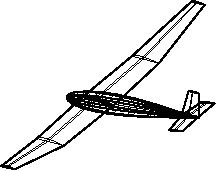
\includegraphics[width=\textwidth]{../figures/geometry_concept-crop.pdf}
        \caption{Concept-level geometry representation, corresponding to the raw data structures within the AeroSandbox geometry stack.}
        \label{fig:geometry_concept}
    \end{subfigure}
    \begin{subfigure}{0.32\textwidth}
        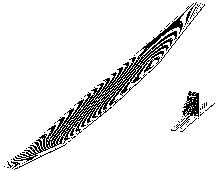
\includegraphics[width=\textwidth]{../figures/geometry_mean_camber-crop.pdf}
        \caption{Mean camber line degenerate geometry representation, which is used during VLM analysis.}
        \label{fig:geometry_mean_camber}
    \end{subfigure}
    \begin{subfigure}{0.32\textwidth}
        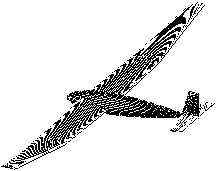
\includegraphics[width=\textwidth]{../figures/geometry_panel-crop.pdf}
        \caption{3D panel degenerate geometry representation, which can be used in other aerodynamic analyses.}
        \label{fig:geometry_panel}
    \end{subfigure}
    \caption{Illustration of several possible degenerate geometry representations produced by the AeroSandbox geometry stack. This removes the need for individual disciplinary analyses to re-implement their own meshing tools, creating a clearer API for new analysis tool development.}
    \label{fig:degen_geometry}
\end{figure}

\subsubsection{Solution Methodology Considerations}

With meshing complete, the governing system of equations described in Section \ref{sec:vlm_theory} can be implemented. Within the context of a code transformations framework, an interesting question is whether this system should be solved explicitly or implicitly. To clarify the difference here:

\begin{itemize}
    \item In an \textbf{explicit} formulation, the matrix and right-hand-side vector of the linear system of equations are explicitly constructed within the analysis code, and the system is solved using a direct solver. In the context of a broader optimization problem encompassing such a model, this means that a) the system of governing equations is solved exactly at each iteration, and b) no optimization variables or constraints are added to the solve.

    \item In an \textbf{implicit} formulation, the horseshoe vortex strengths are posed as optimization variables, and the governing equations are implemented in residual form and constrained (in the top-level optimzation problem) to be driven to zero. This is analogous to a simultaneous-analysis-and-design MDO problem formulation (shown in Figure \ref{fig:sand}). Here, the matrix and right-hand-side vector of the linear system are never explicitly constructed within the analysis code (though of course, the optimization problem constraint Jacobian will essentially compute this same information). In the context of a broader optimization problem encompassing such a model, this means that a) the system of governing equations is solved approximately at each iteration, and b) optimization variables and constraints are added to the solve.

\end{itemize}

Both methods have advantages. The principal advantage of the explicit formulation is that incorporating this into a design optimization framework can yield more stable convergence, since ``correct'' (i.e., zero-residual) solutions are guaranteed at each iteration. This can be especially important in the context of a multidisciplinary optimization problem, where this VLM analysis might be combined with other analyses. Here, a fully coupled implicit system might become numerically unstable (e.g., numerically-stiff), leading to convergence difficulties.

On the other hand, the implicit formulation has the potential to be much faster, in the context of a broader optimization problem. This is because the optimizer is solving for primal feasibility (i.e., constraint violation) and dual feasibility (i.e., optimality conditions) simultaneously. An intuitive way to think about this is that the optimizer is not wasting CPU cycles by solving the analysis accurately during early iterations, when the solution is far from the optimum. Instead, the optimizer is solving the analysis just enough to ensure that the constraints are satisfied, and then moving on to the next iteration. This can lead to significant speedups (up to an order of magnitude, in the author's experience) in the context of a broader optimization problem, especially when the analysis is expensive to solve.

There are also some cases where this implicit solution can be favorable in augmented analyses. For example, if a panel method is coupled with an integral boundary layer model (e.g., in XFoil), solving the problem as a coupled system rather than a segregated disciplinary solve can resolve singularity issues that might otherwise appear \cite{drela_xfoil_1989, drela_viscousinviscid_1987, ranneberg_viiflow_2019, fidkowski_coupled_2022, zhang_threedimensional_2022}.

In the case of the present VLM implementation, both formulations are offered, with the explicit solution being the default. This is because the explicit solution is more stable and easier to debug, and because the VLM analysis is relatively inexpensive to solve. However, the implicit solution is also available, and can be used if the user desires faster convergence in the context of a broader optimization problem.

\subsection{Example Results}

Figure \ref{fig:vlm} shows the results of a VLM analysis performed using AeroSandbox, using a generic glider design and a prescribed aerodynamic operating point. At the moderately high paneling resolution shown here ($N=700$ panels), solution takes about 0.25 seconds on a laptop-grade CPU. The surface color shows the vortex strength (or equivalently, $\Delta C_p$ across the wing), while the streamlines show the flow field.

\begin{figure}[h]
    \centering
    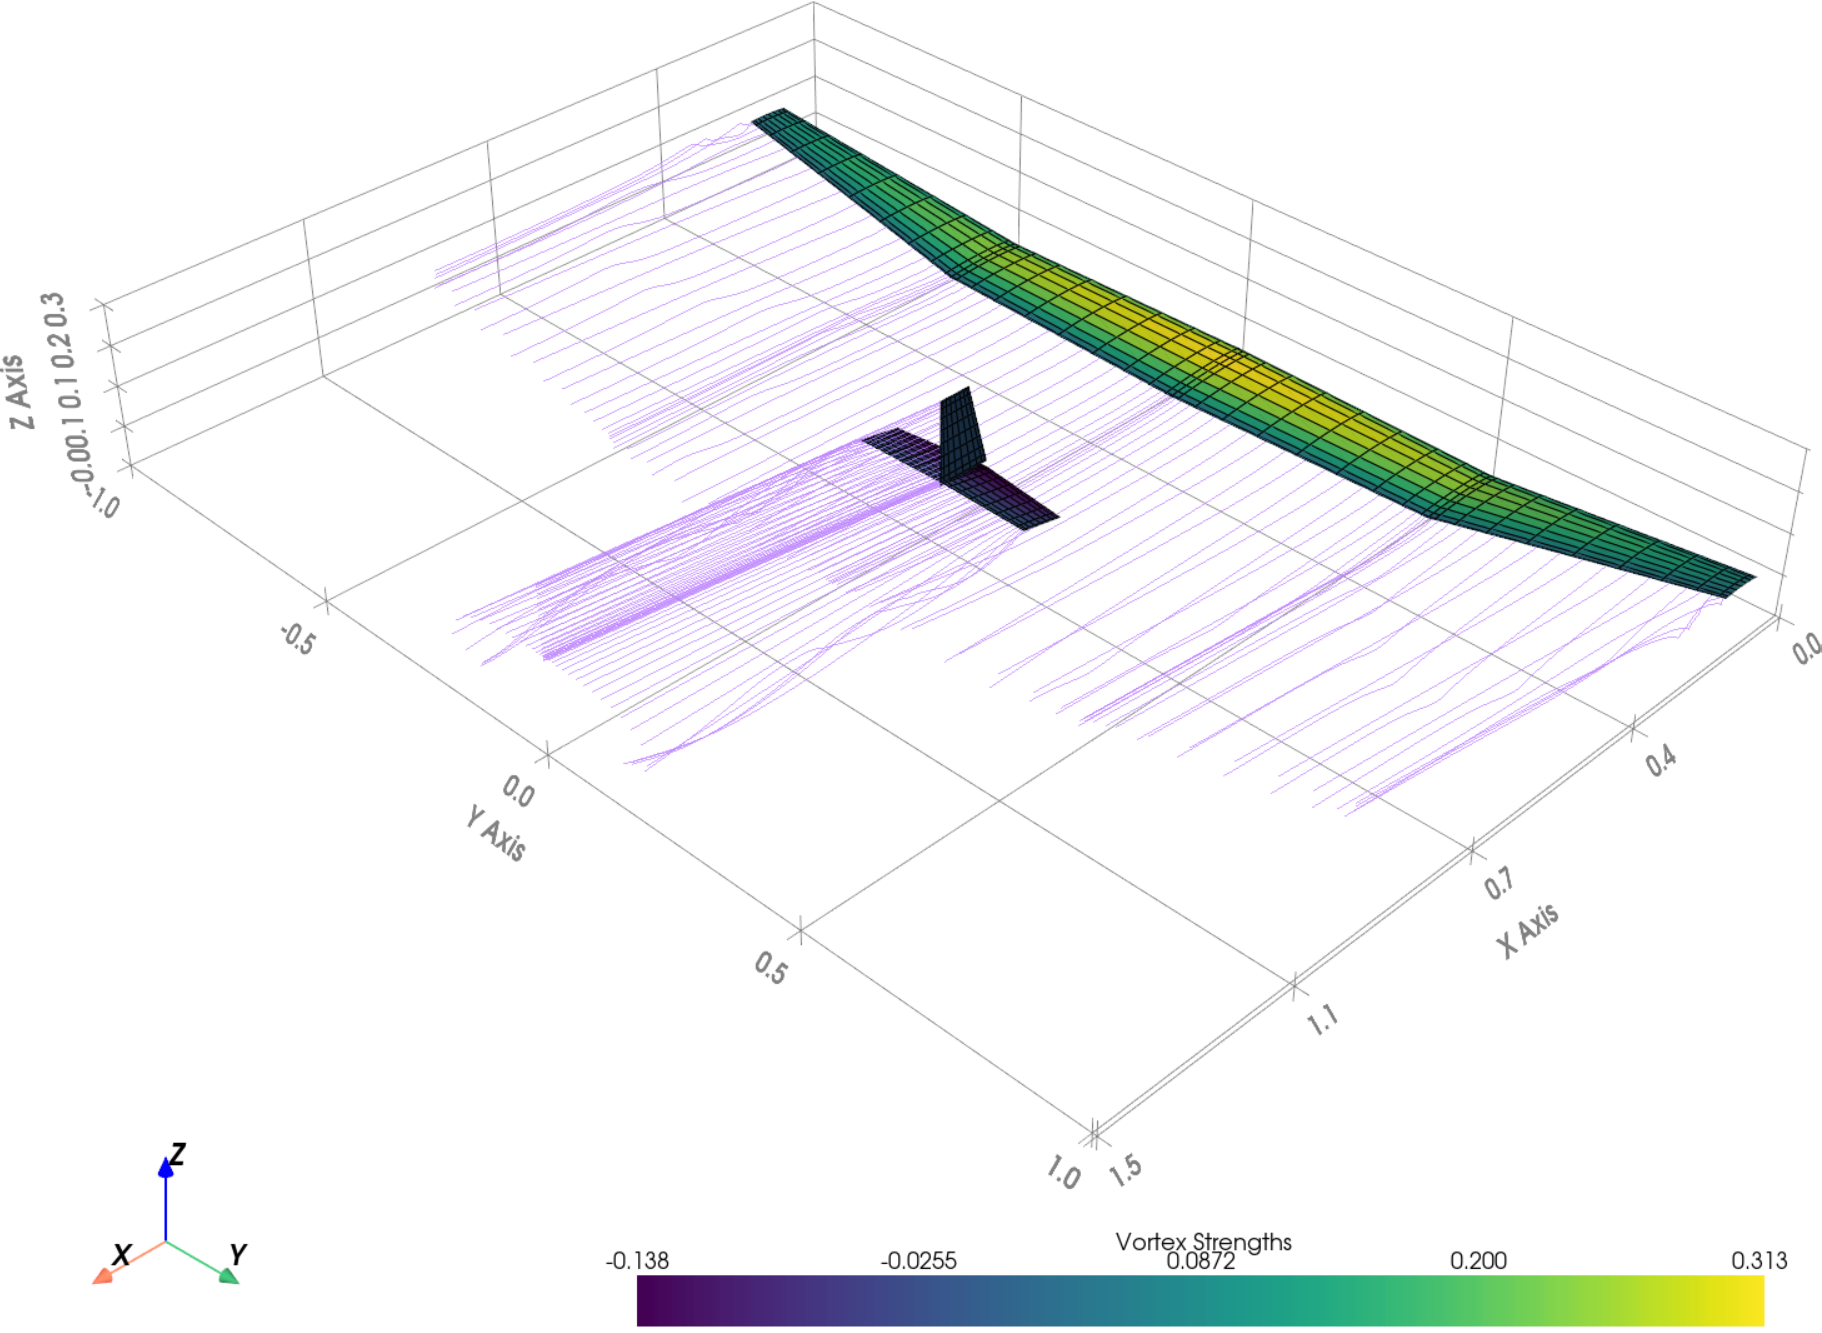
\includegraphics[width=\textwidth]{../figures/vlm.png}
    \caption{AeroSandbox VLM analysis results for a simple glider geometry at a prescribed aerodynamic operating point. Surface color shows the vortex strength (or equivalently, $\Delta C_p$ across the wing). Streamlines show the flow field.}
    \label{fig:vlm}
\end{figure}

Validation results for this VLM analysis are shown later in Section \ref{sec:aero_validation}, where the VLM can be cross-compared not only against external tools but also against the other plug-and-play aerodynamic analyses developed in this chapter. Notably, while the VLM method is quite accurate for computing induced drag, it has no mechanism to compute profile drag without augmentation by another aerodynamic method, like the buildup described in Section \ref{sec:aerobuildup}; hence, the VLM method should not be used by itself for performance analysis. It is, however, more than adequate for flight dynamics analysis, as there are few other low-fidelity aerodynamics methods that handle local velocity effects (e.g., dynamic derivatives, aerodynamic damping) as readily.

\subsection{Aerodynamic Shape Optimization}

To demonstrate how this VLM tool can be incorporated into a broader optimization problem, we can formulate a classic aerodynamic shape optimization problem and compare our result to a known solution.

Here, we aim to find the minimum-induced-drag wing planform, by optimizing a wing's chord distribution. We assume:

\begin{itemize}[noitemsep]
    \item A fixed total lift
    \item A fixed wing area
    \item A fixed span
    \item An untwisted, uncambered, unswept, thin, planar wing
    \item Potential flow (inviscid, incompressible, irrotational, and steady)
\end{itemize}

For this fixed-span, fixed-lift case, theory shows that the minimum-induced-drag wing has an elliptical lift distribution. With the additional assumptions above, the corresponding minimum-induced-drag wing will also have an elliptical \emph{chord} distribution \cite{anderson_fundamentals_2009}.

This problem can be posed in AeroSandbox syntax using the plug-and-play VLM analysis model described in the previous section. We supply an initial guess of a simple rectangular (i.e. untapered) wing, and optimize the chord distribution. We do not know the correct angle of attack $\alpha$ to achieve our specified lift coefficient \emph{a priori}, so this becomes an additional optimization variable. The VLM is implemented, here using just one spanwise panel for each unknown chord variable—typically, a higher resolution ($\sim 4$ panels per optimization variable) would be used for numerical stability, but this is used to demonstrate numerical robustness of the implementation here.

Surprisingly, the entire optimization problem can be written in less than 40 lines of code, allowing it to be shown in its entirety in Listing \ref{lst:vlm_optimization}. This serves as a good illustration of the motivation behind developing these plug-and-play models for a code transformations framework—the modularity allows complex optimization problems to be posed with minimal code.

\begin{listing}[H]
    \begin{minted}{python}
import aerosandbox as asb
import aerosandbox.numpy as np

opti = asb.Opti()  # Initialize an optimization environment.

N = 16  # Spanwise resolution
y = np.sinspace(0, 1, N, reverse_spacing=True)  # Spanwise locations along the wing.
chords = opti.variable(init_guess=1 / 8, n_vars=N, lower_bound=0)  # Chord dist.
wing = asb.Wing(  # Defines the wing geometry.
    symmetric=True,
    xsecs=[  # Cross sections ("XSecs") of the wing
        asb.WingXSec(
            xyz_le=[  # Location of each cross-section's leading edge
                -0.25 * chords[i],  # This keeps the quarter-chord-line straight.
                y[i],  # Our (known) span locations for each section.
                0
            ],
            chord=chords[i],
        )
        for i in range(N)
    ]
)

aero = asb.VortexLatticeMethod(  # Compute aerodynamics using the VLM analysis
    airplane=asb.Airplane(wings=[wing]),  # The geometry to analyze
    op_point=asb.OperatingPoint(  # Aerodynamic operating condition
        velocity=1,  # A fixed velocity; unimportant due to nondimensionalization.
        alpha=opti.variable(init_guess=5, lower_bound=0, upper_bound=30)  # Angle of attack
    ),
    spanwise_resolution=1,  # Uses one panel per wing cross-section
).run()

opti.subject_to([
    aero["CL"] == 1,  # We want a fixed lift coefficient
    wing.area() == 0.25,  # We want a fixed wing area
])

opti.minimize(aero["CD"])
sol = opti.solve()
    \end{minted}
    \caption{AeroSandbox code to optimize the chord distribution of a wing to minimize induced drag.}
    \label{lst:vlm_optimization}
\end{listing}

The optimization problem is solved to tolerance within 18 IPOPT iterations, corresponding to around 10 seconds of wall-clock time on a laptop CPU. This yields the wing geometry shown in Figure \ref{fig:vlm_opt}, which is indeed elliptical in chord distribution. To confirm, the chord distribution can be directly compared to an elliptical distribution as shown in Figure \ref{fig:vlm_opt_compare}. Very slight differences appear due to numerical discretization, but as panel resolution is increased, these results converge.

\begin{figure}[h]
    \centering
    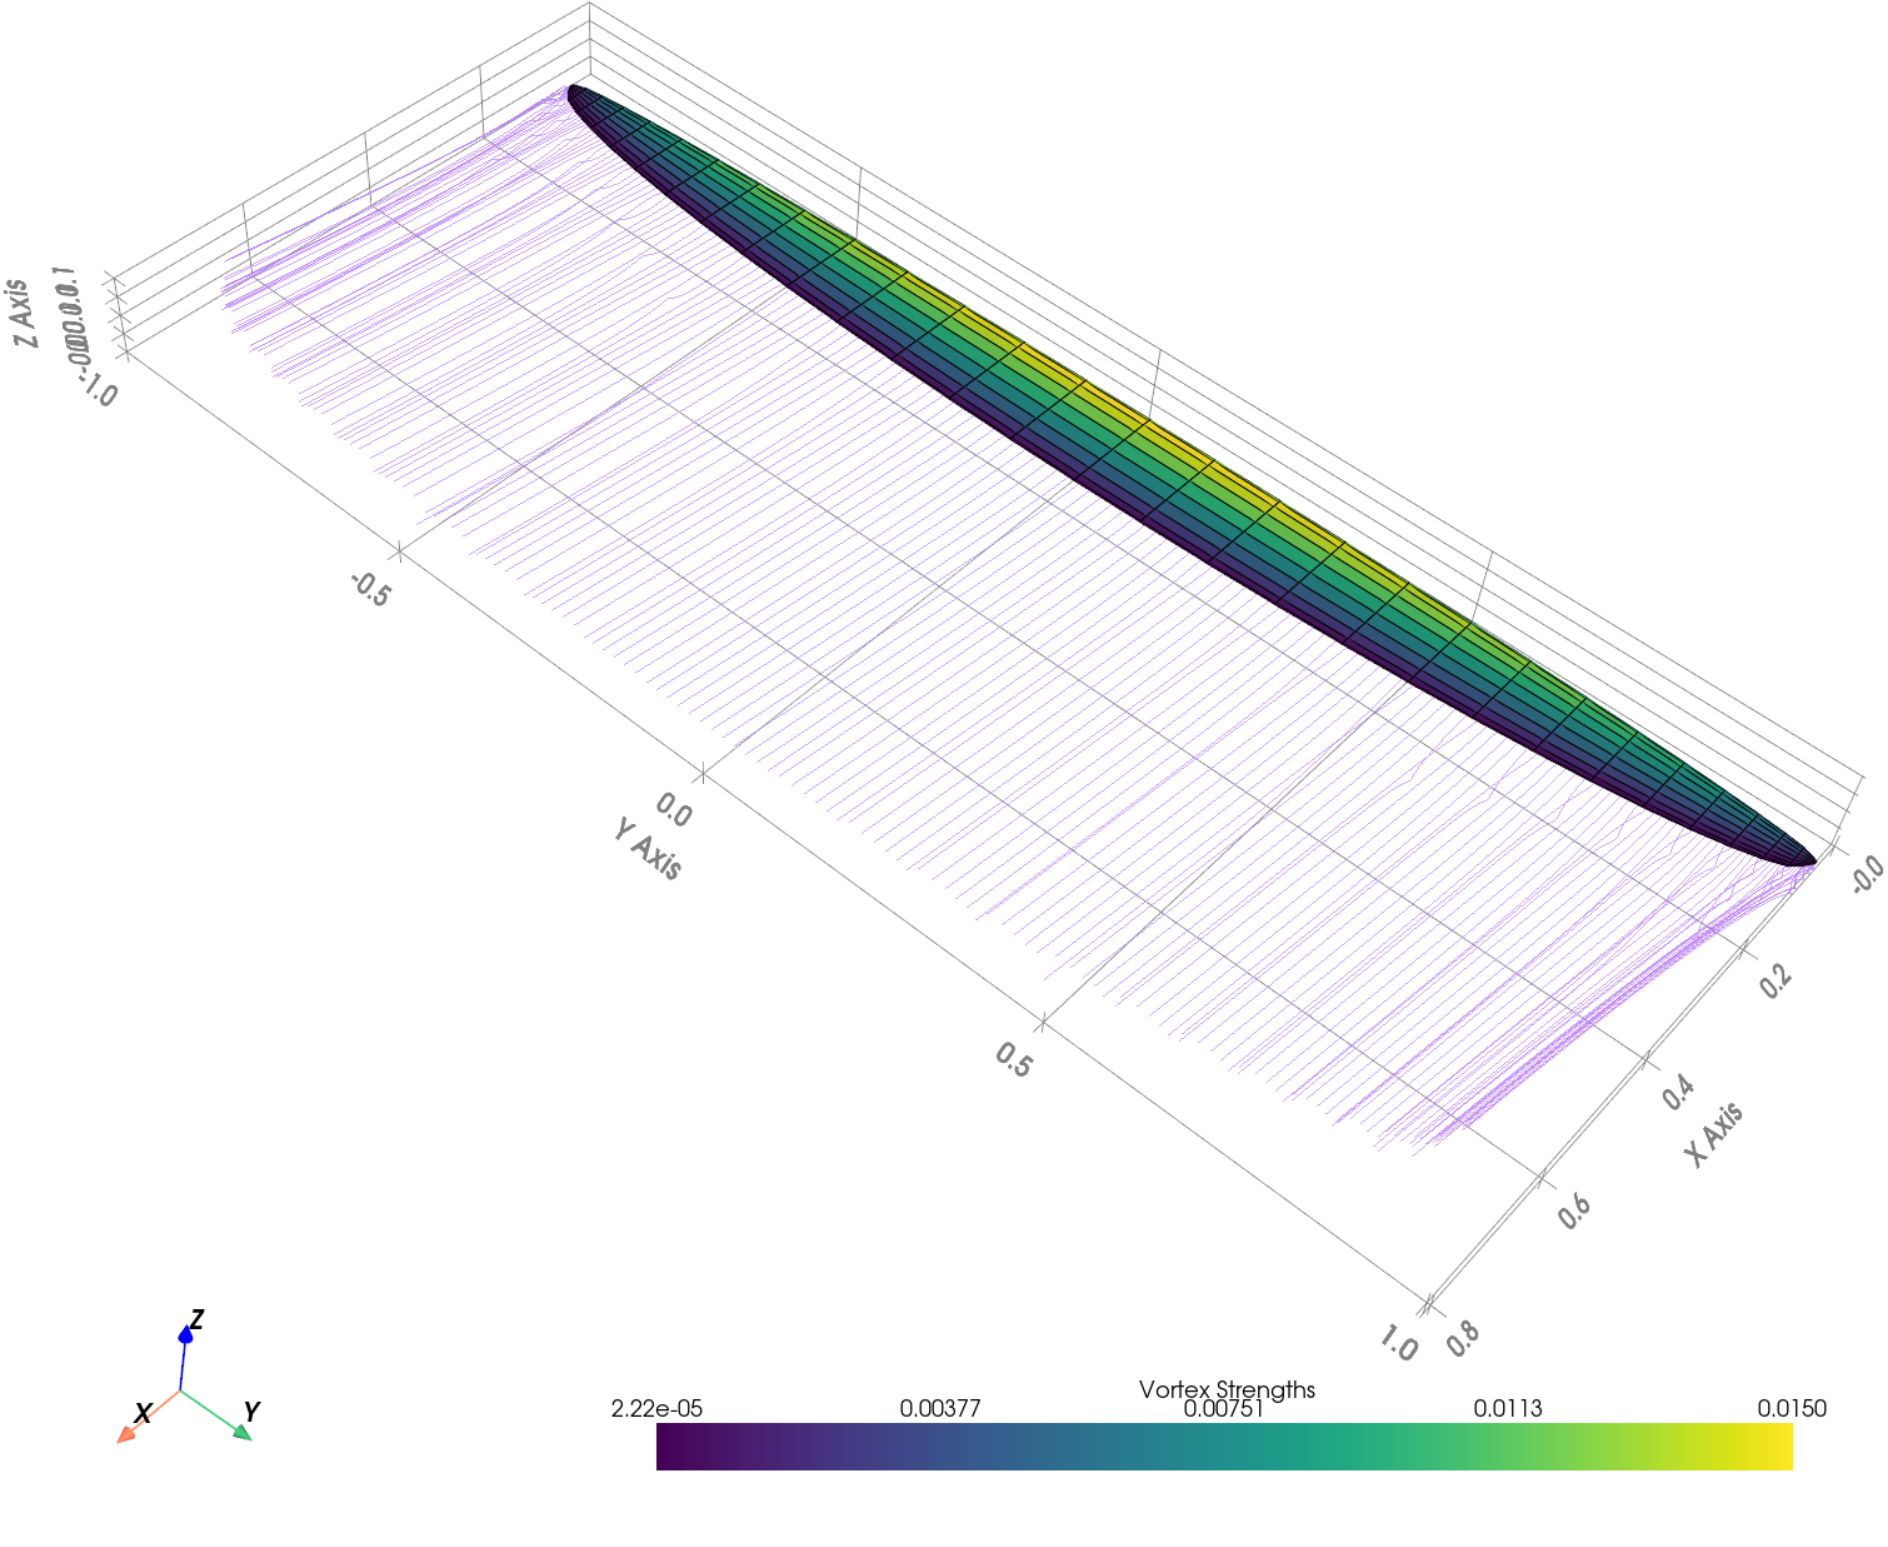
\includegraphics[width=\textwidth]{../figures/vlm_opt.png}
    \caption{Result of the AeroSandbox VLM analysis-based aerodynamic shape optimization problem. The optimized wing has an elliptical chord distribution.}
    \label{fig:vlm_opt}
\end{figure}

\begin{figure}[h]
    \centering
    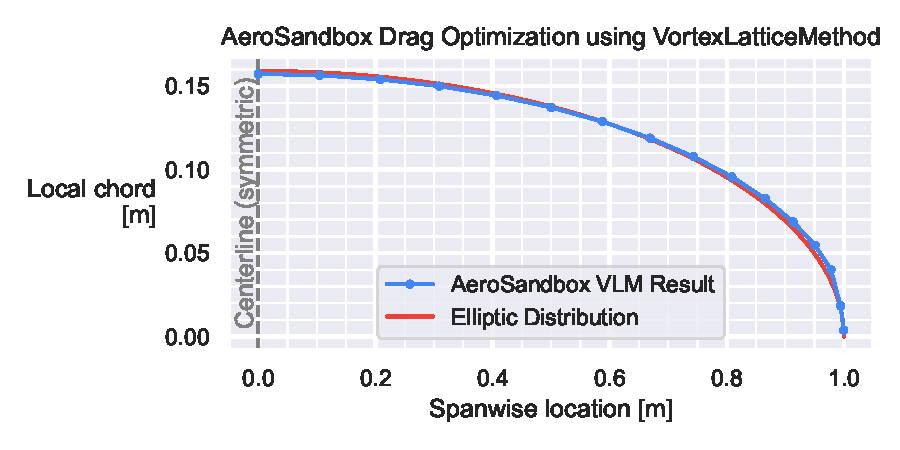
\includegraphics[width=\textwidth]{../figures/vlm_opt_compare.pdf}
    \caption{Comparison of the optimized chord distribution to the theoretical elliptical chord distribution.}
    \label{fig:vlm_opt_compare}
\end{figure}

\section{Nonlinear Lifting Line Aerodynamics Analysis}

\subsection{Method Overview}



%

% TODO sec:aero_validation
% TODO sec:aerobuildup